\restylefloat{table}
  \chapter{Marco Te\'{o}rico}
  \label{chap:cap1}
    \section {Sistemas de almacenamiento}
    
Definici\'{o}n

% expandir
Los sistemas de almacenamiento son importantes puesto que guardan los datos del usuario.

\subsection {Clasificaci\'{o}n por tipo de medio}

\textbf{\\ Medios basados en circuitos \\}

Descripci\'{o}n de los medios, caracter\'{i}sticas, componentes, m\'{e}todo de operaci\'{o}n, similitudes o aplicaciones y capacidad actual.

\begin{itemize}

  \item RAM
  
  Es un medio de almacenamiento vol\'{a}til que se utiliza para guardar datos temporales o como memoria intermedia de un equipo de c\'{o}mputo. Se compone de arreglos de circuitos y tiene una gran velocidad de lectura y escritura comparada con cualquier otro medio de almacenamiento.
  
  \item NVRAM
  
  Es una variante de la memoria RAM donde se almacena la informaci\'{o}n de manera no vol\'{a}til, generalmente su capacidad es peque\~{n}a y este tipo de memoria se utiliza para fines muy especializados, por ejemplo para guardar las configuraciones de algunos sistemas embebidos.
  
  \item ROM
  
  Es una memoria de s\'{o}lo lectura que puede ser grabado una sola vez, generalmente se utilizaba para almacenar firmware de dispositivos o alg\'{u}n programa embebido en hardware que requiere una salida fija para una entrada determinada.
  
  \item EEPROM
  
  Una variante de la memoria ROM donde el contenido puede ser borrado por varios m\'{e}todos, ya sea el\'{e}ctricamente o por medio de la exposici\'{o}n a rayos ultravioleta. En condiciones normales de operaci\'{o}n su comportamiento es similar al de la memoria ROM y se debe entrar en un modo especial para grabar nuevos datos en la misma.
  
  \item FLASH
  
  Una variante m\'{a}s de los medios de almacenamiento basados en circuitos es este tipo de memoria se ha hecho popular en los \'{u}ltimos a\~{n}os gracias a que no depende de partes m\'{o}viles y es de tama\~{n}o peque\~{n}o por lo que es un medio de almacenamiento port\'{a}til y eficiente.
  
  \item SSD
  
  Un medio de almacenamiento relativamente reciente utiliza arreglos de circuitos para guardar la informaci\'{o}n, generalmente se utiliza memoria tipo NAND para mantener los datos y a diferencia de los discos duros no tienen partes m\'{o}viles por lo que son menos propensos a fallos y disipan menos calor.
  
\end{itemize}

\textbf{\\ Medios Magn\'{e}ticos \\}

Este tipo de medios se caracterizan porque el acceso a los datos se realiza mediante un cabezal que lee o escribe el campo magn\'{e}tico impreso en el material que lo guarda. Este tipo de medios es susceptible a fallar si se le expone a campos magn\'{e}ticos, golpes o temperaturas extremas.

\begin{itemize}

  \item Cinta
  
  Las unidades de cinta son medios que almacenan de manera secuencial los datos, por lo que no son de acceso aleatorio. Dentro de sus componentes internos destacan dos carretes que sirven para almacenar la cinta mientras se lee, para acceder datos en una posici\'{o}n anterior es necesario rebobinar la cinta.
  
  Generalmente tienen capacidades que oscilan entre los GB y TB  \cite{b306cc575a86d1e84e6ba100dcfb4417} y son utilizadas para archivar informaci\'{o}n.
  
  \item Discos Flexibles
  
  Este tipo de discos puede acceder de manera aleatoria a los datos almacenados cuentan con un plato magn\'{e}tico rodeado de un material protector contenido en un armaz\'{o}n de pl\'{a}stico que tiene una abertura que permite a la cabeza lectora tener acceso al medio \cite{09678f37a2afcca35133d9a7306744b4}.
  
  Los discos flexibles almacenan los datos dividiendo el plato en circulos conc\'{e}ntricos (pistas) que a su vez se subdividen en arcos (sectores), de esta manera se puede localizar la informaci\'{o}n sabiendo la pista y el sector donde se encuentra \cite{04667739f34ceed8672133b51ada8a35}. Su capacidad oscila entre los cientos de KB hasta llegar a 1.44 MB.
  
  \item Discos Duros
  
  Similar al disco flexible, el disco duro tiene una estructura formada por varios platos, cada uno leido por una cabeza diferente. De manera l\'{o}gica el espacio se organiza en circulos conc\'{e}ntricos (cilindros), platos (cabezas) y arcos (sectores), en modelos modernos se utiliza \emph{Logical Block Addressing} para asignar el espacio.
  
  Parecidos a los discos flexibles, estos medios tienen mayor capacidad y actualmente son el medio primordial de almacenar informaci\'{o}n en los equipos de c\'{o}mputo. A diferencia de los discos flexibles, tienen los componentes mec\'{a}nicos dentro del armaz\'{o}n del disco y pueden almacenar grandes cantidades de informaci\'{o}n gracias a que se apilan varios discos en una estructura cilindrica. Para buscar un dato se debe hacer referencia al plato donde est\'{a}, al sector del disco y a la cabeza de lectura que corresponda.
  
\end{itemize}

\textbf{\\ Medios Magneto-\'{o}pticos \\}

\begin{itemize}

  \item Discos MO (Magneto-optic)
  
  Los discos magneto-\'{o}pticos tienen las bondades de la rapidez de los discos magn\'{e}ticos y la versatilidad de los discos \'{o}pticos, 
  
\end{itemize}

\textbf{\\ Medios \'{O}pticos \\}

Descripci\'{o}n de los medios, caracter\'{i}sticas, componentes, m\'{e}todo de operaci\'{o}n, similitudes o aplicaciones y capacidad actual.

\begin{itemize}

  \item Discos de s\'{o}lo lectura (WORM)
  
  Los discos pre-masterizados (CD-ROM, DVD-ROM, BD-ROM) se graban en las f\'{a}bricas donde se tiene un disco maestro que sirve para transferir los datos al medio final por un proceso de vaciado t\'{e}rmico.
  
  Los discos grabables (CD-R, DVD+R, DVD-R y BD-R) pueden ser grabados mediante un laser al fundir una capa de policarbonato en la superficie inferior del disco para grabar los bits en 1. El formato de los bits generalmente va de acuerdo al est\'{a}ndar ISO-9660.
  
  \item Discos regrabables
  
  Los discos regrabables (CD-RW, DVD+RW, DVD-RW, BD-RE) tienen una ventaja adicional comparados con los discos grabables de una sola vez, es posible borrar la informaci\'{o}n contenida para almacenar nuevos datos en el medio, esto se logra inicializar parcial o totalmente los sectores del disco para que este pueda admitir nuevos datos.
  
\end{itemize}

\textbf{\\ Medios Hologr\'{a}ficos \\}

\begin{itemize}

  \item HVD - Disco Vers\'{a}til Hologr\'{a}fico
  
  Es un nuevo medio de almacenamiento a\'{u}n en desarrollo que ofrece un m\'{e}todo m\'{a}s vers\'{a}til de escribir los datos utilizando un mecanismo hologr\'{a}fico donde dependiendo la manera en la que se leen los datos es la informaci\'{o}n que se obtiene.
  
\end{itemize}

      \subsection {Comparativa de medios de almacenamiento actuales}

\begin{table}[H]
\caption{Comparativa de medios de almacenamiento}{}
\label{tab:comparativa}
\noindent\makebox[\textwidth]{%
% manually center the table in page
\hspace*{-1.1cm}
\begin{tabular}{c|c|c|c|c|c}
%\hline
\multirow{2}{*}{\textbf{Medio}} & \multirow{2}{*}{\textbf{Capacidad}} & \multirow{2}{*}{\textbf{Persistente}} & \textbf{Acceso} & \textbf{Lectura y} & \multirow{2}{*}{\textbf{Vulnerabilidades}} \\
 & & & \textbf{aleatorio} & \textbf{escritura} & \\
\hline
\hline
RAM & MB & 
\includegraphics[keepaspectratio=true, width=10px]{figures/N} & 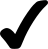
\includegraphics[keepaspectratio=true, width=10px]{figures/Y} & 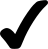
\includegraphics[keepaspectratio=true, width=10px]{figures/Y} & \multirow{5}{*}{Electricidad est\'{a}tica} \\
\cline{1-5}
NVRAM & MB & 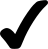
\includegraphics[keepaspectratio=true, width=10px]{figures/Y} & 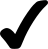
\includegraphics[keepaspectratio=true, width=10px]{figures/Y} & 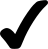
\includegraphics[keepaspectratio=true, width=10px]{figures/Y} &  \\
\cline{1-5}
ROM & MB & 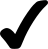
\includegraphics[keepaspectratio=true, width=10px]{figures/Y} & 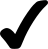
\includegraphics[keepaspectratio=true, width=10px]{figures/Y} & 
\includegraphics[keepaspectratio=true, width=10px]{figures/N} &  \\
\cline{1-5}
EEPROM & MB & 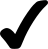
\includegraphics[keepaspectratio=true, width=10px]{figures/Y} & 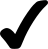
\includegraphics[keepaspectratio=true, width=10px]{figures/Y} & 
\includegraphics[keepaspectratio=true, width=10px]{figures/N} &  \\
\cline{1-5}
FLASH / SSD & GB & 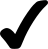
\includegraphics[keepaspectratio=true, width=10px]{figures/Y} & 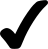
\includegraphics[keepaspectratio=true, width=10px]{figures/Y} & 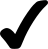
\includegraphics[keepaspectratio=true, width=10px]{figures/Y} &  \\
\hline
Cinta & TB & 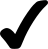
\includegraphics[keepaspectratio=true, width=10px]{figures/Y} & 
\includegraphics[keepaspectratio=true, width=10px]{figures/N} & 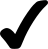
\includegraphics[keepaspectratio=true, width=10px]{figures/Y} & \multirow{3}{*}{Campos magn\'{e}ticos} \\
\cline{1-5}
Disco Flexible & MB & 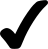
\includegraphics[keepaspectratio=true, width=10px]{figures/Y} & 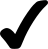
\includegraphics[keepaspectratio=true, width=10px]{figures/Y} & 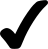
\includegraphics[keepaspectratio=true, width=10px]{figures/Y} &  \\
\cline{1-5}
Disco Duro & TB & 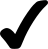
\includegraphics[keepaspectratio=true, width=10px]{figures/Y} & 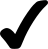
\includegraphics[keepaspectratio=true, width=10px]{figures/Y} & 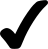
\includegraphics[keepaspectratio=true, width=10px]{figures/Y} &  \\
\hline
\multirow{2}{*}{Disco MO} & \multirow{2}{*}{MB/GB} & \multirow{2}{*}{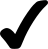
\includegraphics[keepaspectratio=true, width=10px]{figures/Y}} & \multirow{2}{*}{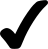
\includegraphics[keepaspectratio=true, width=10px]{figures/Y}} & \multirow{2}{*}{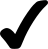
\includegraphics[keepaspectratio=true, width=10px]{figures/Y}} & Campos magn\'{e}ticos\\
 & & & & & Rayaduras \\
\hline
Disco \'{O}ptico & MB/GB & 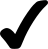
\includegraphics[keepaspectratio=true, width=10px]{figures/Y} & 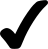
\includegraphics[keepaspectratio=true, width=10px]{figures/Y} & 
\includegraphics[keepaspectratio=true, width=10px]{figures/N} & \multirow{3}{*}{Rayaduras} \\
\cline{1-5}
Disco Regrabable & MB/GB & 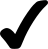
\includegraphics[keepaspectratio=true, width=10px]{figures/Y} & 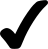
\includegraphics[keepaspectratio=true, width=10px]{figures/Y} & 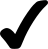
\includegraphics[keepaspectratio=true, width=10px]{figures/Y} &  \\
\cline{1-5}
Disco Hologr\'{a}fico & GB & 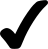
\includegraphics[keepaspectratio=true, width=10px]{figures/Y} & 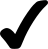
\includegraphics[keepaspectratio=true, width=10px]{figures/Y} & 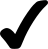
\includegraphics[keepaspectratio=true, width=10px]{figures/Y} & \\
%\hline
\end{tabular}
} % ending of \makebox
\end{table}

  \subsection {Escenarios de falla}

    \begin{itemize}

      \item Da\~{n}o f\'{i}sico del medio

Si el medio de almacenamiento presenta da\~{n}o f\'{i}sico los datos almacenados pueden aparecer incompletos o no se pueden leer.

% Revisar corrompidos

      \item Fallo de componentes internos

Dependiendo del tipo de medio, la falla de componentes internos puede o no ser fatal, por ejemplo, si se tiene un disco \'{o}ptico y falla el lector de discos, basta con reemplazar la unidad para que el disco se pueda leido sin problemas, en cambio si falla el cabezal de un disco duro, ser\'{a} necesario un proceso m\'{a}s complicado y costoso para recuperar la informaci\'{o}n.

% Revisar segunda linea

    \end{itemize}

  \subsection {M\'{e}todos de protecci\'{o}n}

Los m\'{e}todos de protecci\'{o}n de los medios de almacenamiento varian dependiendo de su tipo (consultar la tabla \ref{tab:comparativa} para m\'{a}s informaci\'{o}n)

    \begin{itemize}

      \item Seguro contra escritura
        
El seguro contra escritura previene que los datos sean modificados, puesto que el medio se reconoce como de s\'{o}lo lectura y no es posible escribir en \'{e}l. El uso de este m\'{e}todo es \'{u}til cuando se archivan o respaldan datos porque se busca que estos no sean modificados.

      \item Protecci\'{o}n antiest\'{a}tica y contra campos magn\'{e}ticos
        
Para evitar el da\~{n}o por electricidad est\'{a}tica o campos magn\'{e}ticos en los medios de almacenamiento como cintas o discos duros existen bolsas que evitan que el disco reciba una descarga de electricidad est\'{a}tica y cubiertas especiales para salvaguardar el disco de los campos magn\'{e}ticos.

      \item Protecci\'{o}n contra da\~{n}o f\'{i}sico
       
% ampliar 
El da\~{n}o f\'{i}sico se puede prevenir si se maneja el medio de almacenamiento con precauci\'{o}n y se guarda en un lugar fresco y seco que no tenga exposici\'{o}n directa a la luz solar y que est\'{e} fuera del alcance 

    \end{itemize}

  \subsection {T\'{e}cnicas de respaldo}
  
% gloasario SOHO

En un entorno de hogar u oficina peque\~{n}a (SOHO) el n\'{u}mero de usuario es reducido y tiene la necesidad de almacenamiento centralizado, para resolver este problema varias opciones han aparecido a lo largo de los a\~{n}os:

    \begin{itemize}
      \item Grabar la informaci\'{o}n a discos \'{o}pticos como CDs y DVDs.
      \item Utilizar discos duros o unidades removibles como medio de respaldo.
      \item Compartir directorios a trav\'{e}s de la red para acceder archivos almacenados en equipos remotos.
      \item Utilizar dispositivos de bloque compartidos en red para tener acceso a sistemas de archivos remotos.
      \item Hacer uso de los servicios de almacenamiento en la nube (cloud storage) para guardar los archivos en un sitio remoto y accederlos a trav\'{e}s de Internet.
    \end{itemize}

La descripci\'{o}n de cada elemento se muestra a continuaci\'{o}n:

    \begin{itemize}
    
      \item \textbf{Respaldo en medios \'{opticos}}

% separar en dos parragos, usar comas

Cada soluci\'{o}n tiene sus pros y contras, por ejemplo el guardar informaci\'{o}n en discos \'{o}pticos deja la copia como s\'{o}lo lectura y aunque eso sea bueno para respaldos completos o archivado de datos, no lo es para guardar datos que van a cambiar como documentos que se est\'{a}n editando porque cada vez que se escriba al disco \'{o}ptico se guardar\'{a} una nueva copia del documento en lugar de reemplazar la existente.

      \item \textbf{Respaldo en medios magn\'{e}ticos y unidades port\'{a}tiles}
%uso en masa
Desde la masificaci\'{o}n de los discos duros externos y las unidades port\'{a}tiles se han adoptado como medio de almacenamiento para los datos que cambian mucho. Gracias a que estos medios generalmente son de lectura y escritura, las modificaciones de los archivos pueden guardarse reemplazando la copia original y si un archivo es borrado se recupera el espacio en disco.

Una desventaja del uso de este tipo de medios radica en que se pueden editar tanto la copia local en la computadora como el archivo de respaldo produciendo diferentes versiones y el usuario es quien tiene que decidir que versi\'{o}n del archivo es la que debe considerarse la m\'{a}s actualizada.

      \item \textbf{Recursos compartidos por red}

Cuando se cuenta con una red de computadoras se puede utilizar otro mecanismo para almacenar datos en equipos remotos por medio de recursos compartidos en red. Dependiendo de la configuraci\'{o}n se pueden asignar permisos de s\'{o}lo lectura o lectura-escritura. A diferencia de la copia a unidades port\'{a}tiles, en este caso, se tiene una sola copia de la informaci\'{o}n por lo que no existe posibilidad de encontrar una versi\'{o}n desactualizada de los datos. La gran desventaja de los recursos compartidos entre varios equipos, es que los datos no se pueden acceder cuando el equipo que los almacena se encuentra apagado o con intermitencias de conectividad. Esta soluci\'{o}n funciona mejor cuando los equipos que comparten los recursos est\'{a}n encendidos la mayor\'{i}a del tiempo.

Los protocolos que com\'{u}nmente se utilizan para compartir recursos a trav\'{e}s de la red son NFS y CIFS (samba) siendo el primero el protocolo m\'{a}s utilizado en sistemas tipo UNIX y el segundo se utiliza mayormente en sistemas Windows, aunque se puede utilizar tambi\'{e}n en sistemas UNIX a trav\'{e}s de la suite de herramientas de samba [samba.org]

      \item \textbf{Dispositivos de bloque compartidos por red}

Otra soluci\'{o}n popular en sistemas UNIX es compartir dispositivos de bloque a trav\'{e}s de la red para acceder a discos remotos como si fuesen locales, ejemplos de esto son Network Block Device en GNU/Linux y tecnolog\'{i}as SAN como iSCSI (Internet SCSI) o AoE (ATA over Ethernet), este tipo de soluciones llegan a ser costosas y no se adaptan bien a ambientes como empresas peque\~{n}as u hogares.
    
      \item \textbf{Servicios de almacenamiento en la nube}

En los \'{u}ltimos a\~{n}os los servicios de almacenamiento en la nube han ganado popularidad por ser servicios administrados que no requieren mucha configuraci\'{o}n por parte del usuario. Algunos de estos servicios ofrecen una unidad virtual que se monta en el equipo local para acceder al contenido y agregar o modificar los archivos del usuario, mientras que otros sincronizan las modificaciones locales con el contenido almacenado remotamente y viceversa.

        \textrm{Nube p\'{u}blica}

Los servicios de almacenamiento remotos en Internet son denominados \emph{Almacenamiento de Nube P\'{u}blica}, son \'{u}tiles cuando la velocidad de la conexi\'{o}n se ajusta a la demanda de los usuarios. Dado que los archivos residen en otro lugar, es necesario descargar y subir grandes cantidades de datos al servicio de almacenamiento remoto y si la conexi\'{o}n a Internet no es lo suficientemente r\'{a}pida, la experiencia del usuario se ven afectada.

Com\'{u}nmente este tipo de servicios ofrece menos de 100GB de almacenamiento y al subir o descargar archivos de gran tama\~{n}o la copia es muy lenta.

        \textrm{Nube privada}

Cuando el servicio de almacenamiento se encuentra en la red local, se puede aprovechar de mejor manera, dado que la velocidad de transmisi\'{o}n en una red local es m\'{a}s r\'{a}pida que entre redes separadas. Adem\'{a}s el servicio no est\'{a} disponible para clientes de otras redes por lo que se denomina \emph{Privado}. En este caso los usuarios tienen mejor experiencia y los datos se quedan resguardados en un equipo dentro de la organizaci\'{o}n.

En este tipo de soluciones se pueden tener grandes vol\'{u}menes de datos disponibles para los usuarios, aprovechando la rapidez de la red local para manipular archivos de gran tama\~{n}o.

    \end{itemize}

  \subsection {Arreglos RAID}

El t\'{e}rmino RAID es un acr\'{o}nimo de \emph{Redundant Array of Inexpensive Disks} (Arreglo Redundante de Discos Independientes) \cite{8810bc4904cabf93eede72a03c171b7e} \footnote{Dependiendo de la bibliograf\'{i}a el t\'{e}rmino puede ser tambi\'{e}n referido como \emph{Redundant Array of Inexpensive Disks} (Arreglo Redundante de Discos Baratos).}. Es una tecnolog\'{i}a que se basa en combinar m\'{u}ltiples discos para que se comporten como uno solo. Dependiendo el modo de operaci\'{o}n, ofrece la posibilidad de tomar varios discos y sumar el espacio de almacenamiento o bien replicar los datos escribiendolos en varios discos para tener tolerancia a fallos.

Los arreglos de disco se pueden configurar por tarjetas dedicadas de hardware o mediante configuraci\'{o}n de software en el sistema operativo. En los \emph{arreglos por hardware} el firmware de la tarjeta controladora tiene los algoritmos encargados de leer, escribir y sincronizar los datos, mientras que en los \emph{arreglos por software} el kernel del sistema operativo es el encargado de realizar estas operaciones.

Tipo de arreglos RAID

\begin{itemize}

  \item \textbf{Linear}

En esta variante se combinan dos o mas discos como si fueran uno solo al \emph{concatenar} el espacio y s\'{o}lo se escribir\'{a} al disco 1 si el disco 0 se encuentra lleno.

Para crear el arreglo no importa el tama\~{n}o de los discos. Si se acceden dos archivos que est\'{a}n almacenados en diferentes discos el rendimiento aumenta porque la lectura se realiza en paralelo.

Este m\'{e}todo no ofrece redundancia, por lo que si falla un disco los datos contenidos en este se pierden. Es posible montar el sistema de archivos en un modo especial y recuperar los datos almacenados en los dem\'{a}s discos.

{\large\begin{verbatim}<Falta imagen/>\end{verbatim}}
% http://www.linuxhomenetworking.com/wiki/index.php/Quick_HOWTO_:_Ch26_:_Linux_Software_RAID
% http://nst.sourceforge.net/nst/docs/user/ch14.html

  \item \textbf{RAID 0}

Tambi\'{e}n llamado \emph{Stripe}, organiza los datos en bloques que se reparten en los discos copiando un bloque a cada disco.

Aunque es posible crear el arreglo con discos de diferente tama\~{n}o, se recomienda que sean por lo menos dos discos de la misma capacidad. Gracias a la organizaci\'{o}n de los datos en los discos, estos se acceden en paralelo aumentando la velocidad de lectura y escritura.

No ofrece redundancia porque los bloques se reparten en todos los discos y si uno falla se perder\'{a}n partes de todos los archivos haciendo que el contenido no tenga coherencia.

Diagrama \cite{18b4e676f432f4780a509b508056c779}
{\large\begin{verbatim}<Falta imagen/>\end{verbatim}}

  \item \textbf{RAID 1}
  
Denominado \emph{Mirror}, guarda una copia exacta de los datos en ambos discos. Se requiere un m\'{i}nimo de dos discos de igual tama\~{n}o para hacer este arreglo, si los discos son de diferente capacidad, el espacio del arreglo ser\'{a} el del disco m\'{a}s peque\~{n}o.

Este tipo de arreglo es tolerante a fallos siempre y cuando un solo disco siga funcionando porque contiene una copia exacta de los datos contenidos en los dem\'{a}s medios.

El rendimiento de escritura es menor al que presenta un solo disco porque se deben de hacer copias exactas de la informaci\'{o}n en todos los discos pertenecientes al arreglo.

Diagrama \cite{0a250ce04fb10680f70cb2c3efd365b1}
{\large\begin{verbatim}<Falta imagen/>\end{verbatim}}

  \item \textbf{RAID 5}

En este tipo de arreglo se dividen los datos en bloques como sucede en RAID 0 y adem\'{a}s se calcula un bloque de paridad que sirve para reconstruir los datos si uno de los discos falla.

Esta configuraci\'{o}n de RAID tiene tolerancia a fallos, siempre y cuando no falle m\'{a}s de un disco en el arreglo. Se requieren por lo menos tres discos para hacer el arreglo.

Dado que se calcula la paridad de los bloques de datos , se debe restar el tama\~{n}o de un disco para obtener el espacio m\'{a}ximo utilizable.
  
Diagrama \cite{9397b15f6a384de60446b869f05412af}
{\large\begin{verbatim}<Falta imagen/>\end{verbatim}}

  \item \textbf{RAID 6}

Su funcionamiento es similar al de RAID 5, s\'{o}lo que se calculan dos bloques de paridad para cada bloque de datos.

Esta configuraci\'{o}n de arreglo puede tolerar el fallo de hasta dos discos duros, mismos que se reconstruyen utilizando los bloques de paridad. Se requieren al menos cuatro discos para hacer un arreglo RAID 6.

Las operaciones de escritura tardan mas porque se deben calcular dos bloques de paridad, las operaciones de lectura no se ven afectadas.
  
Diagrama \cite{9e2f3e1ba21ce971703a62c6217946ae}
{\large\begin{verbatim}<Falta imagen/>\end{verbatim}}
  
\end{itemize}

Arreglos anidados

Los arreglos anidados \cite{3e1f0dad689a7971f226a3ded845ae63}

\begin{itemize}

  \item \textbf{RAID 10}

Consiste en un arreglo RAID 0 conformado por dos o m\'{a}s arreglos RAID 1, el sistema operativo detecta la presencia de un solo disco mientras que este se conforma por un arreglo RAID 0 (Stripe) que une los dos arreglos RAID 1 (Mirror).

Si un disco de alg\'{u}n arreglo RAID 1 falla, este entra en modo degradado y el funcionamiento del arreglo RAID 0 no se ve afectado \footnote{Salvo por la perdida de rendimiento en el arreglo.}, si fallan dos discos del mismo arreglo RAID 1 el arreglo RAID 0 pierde los datos. Se requieren por lo menos cuatro discos para hacer esta configuraci\'{o}n.

RAID 01... Diagrama \cite{3638d46cd02c0cd72e333c6d6f8f9608}
\begin{verbatim}
        SO
         |
       RAID 0
     |        |
  RAID 1     RAID 1
  |    |     |    |
HDD1  HDD2 HDD3  HDD4
\end{verbatim}
  

  \item \textbf{RAID 01}

Se compone por un arreglo RAID 1 que replica los datos contenidos en dos arreglos RAID 0. Se requiere un m\'{i}nimo de cuatro discos para hacer esta configuraci\'{o}n.

Si falla uno o dos discos del mismo arreglo RAID 0, todo el arreglo se pierde y el arreglo RAID 1 entra en modo degradado sin perder los datos, si adem\'{a}s falla un disco de otro arreglo RAID 0 todos los datos se pierden.
  
RAID 10... Diagrama \cite{9b286bf9442c2cf4d1e02ddf7322c92b}
\begin{verbatim}
        SO
         |
       RAID 1
     |        |
  RAID 0     RAID 0
  |    |     |    |
HDD1  HDD2 HDD3  HDD4
\end{verbatim}
  
\end{itemize}

      \subsection {Comparativa de tipos de arreglo RAID}

\begin{table}[H]
\caption{Comparativa de arreglos RAID}{}
\label{tab:comparativa}
\noindent\makebox[\textwidth]{%
% manually center the table in page
\hspace*{-1.1cm}
\begin{tabular}[c]{c|c|c|c|c|p{5.95cm}}
%\hline
\textbf{Tipo} & \textbf{Redundancia} & \textbf{Paridad} & \textbf{Discos} & \textbf{Capacidad \'{u}til} & \multicolumn{1}{c}{\textbf{Ventajas}} \\
\hline \hline
\multirow{3}{*}{Linear}  & 
\includegraphics[keepaspectratio=true, width=10px]{figures/N} & 
\includegraphics[keepaspectratio=true, width=10px]{figures/N} & 2+ & Todos los discos & Los datos se escriben en el siguente disco cuando el actual se llena. \\
\hline
\multirow{2}{*}{RAID 0}  & 
\includegraphics[keepaspectratio=true, width=10px]{figures/N} & 
\includegraphics[keepaspectratio=true, width=10px]{figures/N} & 2+ & Todos los discos & Los bloques se escriben en paralelo en los discos. \\
\hline
\multirow{2}{*}{RAID 1}  & 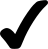
\includegraphics[keepaspectratio=true, width=10px]{figures/Y} & 
\includegraphics[keepaspectratio=true, width=10px]{figures/N} & 2+ & 1 Disco  & Se tiene una copia exacta de los datos en los discos. \\
\hline
RAID 5  & 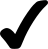
\includegraphics[keepaspectratio=true, width=10px]{figures/Y} & 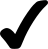
\includegraphics[keepaspectratio=true, width=10px]{figures/Y} \tiny{simple} & 3+ & 2 Discos & Tolera el fallo de un disco. \\
\hline
RAID 6  & 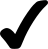
\includegraphics[keepaspectratio=true, width=10px]{figures/Y} & 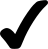
\includegraphics[keepaspectratio=true, width=10px]{figures/Y} \tiny{doble} & 4+ & 2 Discos & Tolera el fallo de hasta dos discos. \\
\hline
RAID 10 & 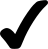
\includegraphics[keepaspectratio=true, width=10px]{figures/Y} & 
\includegraphics[keepaspectratio=true, width=10px]{figures/N} & 4+ & 2 Discos &  \\
\hline
RAID 01 & 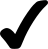
\includegraphics[keepaspectratio=true, width=10px]{figures/Y} & 
\includegraphics[keepaspectratio=true, width=10px]{figures/N} & 4+ & 2 Discos &  \\
%\hline
\end{tabular}
} % ending of \makebox
\end{table}

    \section {Appliances}

Definici\'{o}n de appliance \cite{74e586f4d341588a0bcc6273c524d8f5}

Tipos de Appliance

\begin{itemize}

  \item Hardware
  
Los appliances de hardware son sistemas especializados dise\~{n}ados para realizar tareas espec\'{i}ficas, el fabricante los distribuye en servidores independientes y para agregar funcionalidades o aumentar la capacidad puede ser necesario comprar una licencia adicional o incluso comprar un nuevo equipo que realice esta nueva funcion.

Regularmente tienen una interfaz web para administraci\'{o}n, algunos integran un shell para realizar las funciones conectandose a trav\'{e}s de ssh y en otros casos integran adem\'{a}s soporte para SNMP.
\cite{dcd32ad713054f2f67fbcd17c0900928}

  \item Software
  
Los appliances de software pueden ser distribuidos en paquetes descomprimibles (tarballs) que contienen el instalador y todos los progamas necesarios para que funcione la soluci\'{o}n.

Estos integran s\'{o}lo la interfaz web, puesto que se ejecutan en un equipo existente y son independientes del shell o el soporte SNMP que se tenga en el mismo.
%Los appliances de software son programas descomprimibles o imagenes ISO instalables
[bitnami.org]
\cite{4cb5bff4c029d86b328a2126e8a3060f}
  
  \item Virtual 

Los appliances virtuales son im\'{a}genes de m\'{a}quinas virtuales espec\'{i}ficamente dise\~{n}adas para un ambiente de virtualizaci\'{o}n que integran la funcionalidad de los appliances de hardware dentro de un equipo virtual. Para aumentar la capacidad de este tipo de equipos se pueden instalar m\'{a}s instancias de la m\'{a}quina virtual para procesar en paralelo las peticiones de los usuarios.
\cite{314f38cbb73bf967a21191775959cf1d}
  
\end{itemize}

\section {Seguridad Inform\'{a}tica}
    
Definici\'{o}n de seguridad inform\'{a}tica

  \subsection {Principios de seguridad inform\'{a}tica}
% http://www.oregon.gov/DAS/CIO/ISRC/pages/intro_basics.aspx
% http://csrc.nist.gov/publications/nistpubs/800-14/800-14.pdf

\begin{itemize}

  \item \textbf{Confidencialidad}

Este principio busca conservar los datos \'{u}nicamente para la persona que est\'{a} destinada a leerlos.

Por ejemplo, al cifrar un correo electr\'{o}nico o un archivo se garantiza que s\'{o}lo ser\'{a} visto por la persona que tenga los medios para descifrarlo (ya sea una llave privada o una contrase\~{n}a).

  \item \textbf{Integridad}

Este principio busca que la informaci\'{o}n no pueda ser alterada, ya sea por fallos en el medio de almacenamiento o modificaciones no autorizadas.

Por ejemplo, al firmar un archivo o un correo electr\'{o}nico la firma s\'{o}lo pasar\'{a} la prueba de verificaci\'{o}n si el mensaje est\'{a} integro, de lo contrario no podr\'{a} ser verificado satisfactoriamente.

  \item \textbf{Disponibilidad}

Este principio dicta que la informaci\'{o}n debe poderse acceder cuando sea necesario o respetando el criterio de los tiempos establecidos.

Por ejemplo, un recurso en linea debe estar disponible siempre para que pueda ser accedido por las personas que har\'{a}n uso de el, en caso de tener horarios de disponibilidad se debe garantizar que el recurso se pueda acceder durante ese periodo.

\end{itemize}

  \subsection {Vulnerabilidades}

Una vulnerabilidad es un fallo en la l\'{o}gica o una situaci\'{o}n que se da en condiciones especiales con la que un programa o proceso realiza tareas para las que no fue originalmente destinado. Cuando se alcanzan estas condiciones y se modifica la ejecuci\'{o}n del programa se dice que se ha \textit{explotado} la vulnarabilidad.

% http://www.first.org/cvss/cvss-guide.html
% http://nvd.nist.gov/cvss.cfm?calculator&adv&version=2
% http://www.first.org/cvss
% http://cve.mitre.org/

  \subsection {Hardening}

Se denomina \textit{hardening} al proceso de reforzar las configuraciones del sistema operativo y las aplicaciones para reducir la posibilidad de que una vulnerabilidad se presente.

El hardening se puede realizar en diferentes partes del sistema operativo como:

\begin{itemize}
  \item Configuración de acceso físico
  \item Configuración de inicio
  \item Configuración de acceso remoto
  \item Configuración de las aplicaciones
\end{itemize}

\section {GNU/Linux}
  \subsection {Historia}
  \subsection {Uso de GNU/Linux en la industria}
  \subsection {Distribuciones de GNU/Linux}
  \subsection {Debian GNU/Linux}
\section {Protocolo HTTP}
  \subsection {HTTPS - HTTP over SSL}
  \subsection {WebDAV}
\section {Protocolo LDAP}
  \subsection {Directorio de usuarios}
\section {Protocolo SSH}
  \subsection {SCP - Secure Copy}
  \subsection {SFTP - Secure FTP}
  \subsection {SSHFS - Secure Shell Filesystem}

